\chapter{The Bring-Up of The Collective: From Simulation to Reality}

While Chapter~9 detailed how a localized group of Stewards can bootstrap a single physical Node, we must also address the macro-level genesis of The Collective itself. How does the overarching software stack come into existence, and how does it reach critical mass across millions of people before a single physical solar panel is ever deployed?

The answer lies in blurring the line between digital entertainment and physical infrastructure. The Collective is brought to life through a staged transition from a simulated video game into a real-world thermodynamic engine. It is an open invitation disguised as an engaging simulation, bridging the psychological chasm between late-stage capitalist reliance and sovereign mutual resilience.

\section{Building the Stack and Oasis via Scenario-Driven Development}

The Genesis of The Collective begins purely in software. The Sovereign Stack is developed in tandem with \textit{Oasis}, a massively multiplayer simulation environment. 

This development is strictly governed by Scenario-Driven Development (ScDD). The goal of ScDD is twofold. First, it drives the simulation to mathematically model The Collective's ability to manage the Local Commons---simulating the thermodynamic energy requirements of an eco-village, the water retention of specific soil types, and the systemic health of the bioregion \parencite{jorgensen2001thermodynamics}. 

Second, it simulates \textit{Legacy System Pressure}. A Node does not exist in a utopian vacuum; it is born under the crushing weight of late-stage capitalism. ScDD actively models hostile external shocks: fiat hyperinflation, supply chain collapses, aggressive regulatory inspections by municipal bodies, and utility monopoly shutoffs. By wiring the Sovereign Stack's ledgers (Layer~3) and Orchestrator (Layer~4) directly into these hostile scenarios within Oasis, developers prove mathematically that the architecture is not only viable in theory, but resilient enough to survive the dying thrashes of the legacy world before it is ever deployed in reality.

Crucially, ScDD does not model physical thermodynamics in isolation. It incorporates the psychological and sociological friction of communal life: chore fatigue, interpersonal conflict, seasonal affective strain, and collaborative crisis coordination. If a simulated governance protocol or microgrid allocation formula causes virtual communities to implode from internal resentment, the protocol is refined in software before human lives depend upon it.


\section{The Four Heritage Pillars of the Oasis Engine}
\label{sec:oasis-heritage}

To achieve both compelling gameplay and uncompromising cybernetic fidelity, the Oasis Game Design Document (GDD) deliberately departs from standard video game tropes. There are no arbitrary hit-points, cosmetic microtransactions, or artificially balanced encounters. Instead, Oasis synthesizes the mechanical DNA of four foundational simulation frameworks:

\begin{enumerate}
    \item \textbf{Dwarf Fortress: Thermodynamics and Emergent Psychology:} Oasis completely rejects superficial, linear ``need bars'' (Hunger, Energy, Social) that characterize mainstream life simulators. Such bars create agents with instant amnesia who are cured of existential grief by a slice of pizza. Oasis implements a deep cognitive architecture:
    \begin{itemize}
        \item \textit{32-Slot Episodic Memory Ring Buffer:} Every agent maintains a bounded ring buffer of significant lived experiences. Traumatic events (e.g., an aggressive code enforcement raid or an inverter fire) create permanent, high-salience memories that resist FIFO eviction. Agents experience spatial flashbacks and localized anxiety when traversing the coordinates of past trauma.
        \item \textit{Dual-Timescale Stress Integration:} Stress accumulates under a non-linear Lyapunov damping equation. Acute emotional shocks decay rapidly ($\tau_{\mathrm{acute}} = 30$\,s), while chronic unresolved pressure integrates over weeks ($\tau_{\mathrm{baseline}} = 7$\,days), driving authentic psychological breakdowns (melancholia, withdrawal, tantrums) or inspired creative trances (``Strange Moods'' leading to masterwork artisanal innovations).
    \end{itemize}

    \item \textbf{The Sims: Indirect Founder Agency and Embodiment:} Conventional colony simulators position the player as an omniscient digital dictator wielding an RTS ``god cursor,'' ordering pawns into backbreaking labor without ethical friction. Oasis rejects this authoritarian pattern. The player guides \textit{Founder 01}, a mortal human steward with bounded physical stamina:
    \begin{itemize}
        \item \textit{The Cadastral Slate:} The player interacts via an in-world tablet, suggesting architectural blueprints and enqueuing advisory chores. Founder 01 processes this queue through an internal deliberative utility evaluator based on hydration, caloric energy, emotional reserves, and core ethical convictions.
        \item \textit{Gibsonian Environmental Affordances:} The player influences the community primarily by altering the physical environment. Lighting a rocket mass heater naturally gathers shivering citizens to converse; simmering vegetable stew at dusk convenes the settlement into the communal kitchen for spontaneous social bonding.
        \item \textit{Autonomous Moral Refusal:} Founder 01 is an autonomous being. Directives that violate core ethics (e.g., dumping toxic battery electrolyte into the aquifer) trigger outright moral refusal: Founder 01 drops their tools, defies the cursor, and telegraphs their protest in-world.
    \end{itemize}

    \item \textbf{Cities: Skylines: Macroscopic Logistics and Leeching the Legacy:} Traditional city builders spawn settlements upon pristine meadows hooked to infinite, benevolent municipal grids. Oasis places the player within the decaying, extractive infrastructure of late-stage industrial society. The core macroscopic loop is \textit{Leeching the Legacy}:
    \begin{itemize}
        \item \textit{Parasitic Scavenging:} The nascent settlement survives by siphoning power from aging high-voltage drops via inductive clamps, tapping abandoned municipal water mains, and quarrying broken asphalt for urbanite foundations.
        \item \textit{Severing the Umbilical Cord:} The ultimate progression arc is not endless urban sprawl, but the systematic depaving of asphalt, regeneration of living soil, and thermodynamic closure of the local loop until the legacy utility umbilical cord is permanently cut.
    \end{itemize}

    \item \textbf{Sovereign Stack Multiplayer and the Boundary Interface:} Oasis contains zero custom peer-to-peer networking code, zero WebRTC socket spaghetti, and zero centralized game servers. All multiplayer interaction routes strictly through the Sovereign Stack via the UHAI shared-memory IPC boundary:
    \begin{itemize}
        \item \textit{The Boundary Interface:} The perimeter of the player's parcel is a stochastic boundary subject to legacy shocks arriving via an inhomogeneous Poisson process with intensity:
        \begin{equation}
            \lambda(t) = \max\left(\lambda_{\min}, \, \lambda_{\mathcal{R}} e^{-\Psi(t)}\right)
        \end{equation}
        \item \textit{Sovereign Attenuation Potential ($\Psi$):} Hostile boundary pressure is deterministically attenuated through three vectors: physical autarky ($\Phi_{\mathrm{infra}}$, such as solar storage and rainwater retention), social cohesion ($\Phi_{\mathrm{social}}$, such as integrating newcomers into trust rings), and cryptographic peer proximity mesh ties ($\Phi_{\mathrm{mesh}}$) with neighboring nodes.
        \item \textit{The Fog of Legacy:} Visually, external unmanaged space is shrouded in volumetric smog illuminated by distant sirens and sodium-vapor lamps. As sovereign infrastructure and mutual aid expand, the fog recedes, opening verdant commons corridors between neighboring parcels.
    \end{itemize}
\end{enumerate}


\section{Launching the Game as an Anti-Extractive Platform Cooperative}

Once the simulation engine achieves mathematical stability under ScDD stress-testing, Oasis is released to the legacy public as an immersive multiplayer video game. 

Crucially, this launch is not a cynical bait-and-switch, nor does it view players as unwitting dupes to be milked for fiat. Social movements built on deception inevitably collapse from internal cynicism. Instead, Oasis is launched as an open, transparent \textit{platform cooperative} and an open invitation to a new civilizational architecture. 

To the mainstream gamer, Oasis appears as a masterpiece of systems design: a breathtakingly detailed ecological and societal simulation where players build, govern, and defend settlements against realistic physical and economic pressures. It is published by an open-source publishing cooperative established under Layer~7 with a strict non-profit asset lock in its charter. Yet, from the very first splash screen, Oasis radically rejects the exploitative practices of platform capitalism \parencite{zuboff2019}:
\begin{itemize}
    \item \textbf{Zero Predatory Monetization:} There are no loot boxes, no gambling mechanics, no predatory microtransactions, and no artificial dopamine treadmill loops designed to induce addiction \parencite{han2015}.
    \item \textbf{Complete Code Transparency:} The core engine, simulation logic, and network protocols are entirely open-source, convivial software \parencite{illich1973}.
    \item \textbf{Transparent Commoning Covenant:} Every player knows that purchasing the game or contributing to maintenance funds is not enriching distant venture capitalists. Revenue collected by the publishing entity flows into an open bioregional commons trust, dedicated exclusively to funding physical hardware, land trusts, and mutual aid infrastructure in real-world communities.
\end{itemize}

Simultaneously, the global player base serves as an immense, voluntary testing ground for the Sovereign Stack. Millions of players stress-test the Semantic Layer's visual interfaces, discover edge-case bugs in BPMN workflow coordination, and experiment with polycentric governance protocols. What would require decades of trial and error in physical institutions is iterated and perfected through joyful, collective digital play.


\section{Georeferenced Matchmaking and Localized Privacy}

A defining feature of Oasis is optional, cryptographically private georeferencing. When a player logs in, they may permit their client to locally reference their physical bioregion. 

Crucially, to preserve absolute cryptographic privacy, \textbf{geodata never leaves the player's local device}:
\begin{itemize}
    \item \textbf{Decentralized Tile Distribution:} Rather than uploading the player's location to a central matchmaking server, the local client determines its bioregional coordinates and downloads the relevant topographical elevation maps, hydrological flow charts, and climatic soil histories as content-addressed tiles over decentralized, local-first protocols (IPFS and Reticulum mesh caches).
    \item \textbf{Speed-of-Light Distance Bounding:} Physical proximity between neighboring players is verified cryptographically without central location tracking. The Sovereign Stack executes hardware-level round-trip challenge-response distance bounding over physical radio:
    \begin{equation}
        d_{AB} \le \frac{c \cdot (\Delta t - t_d)}{2}
    \end{equation}
    where $c$ is the speed of light, $\Delta t$ is the round-trip latency over local physical radio (LoRa or 802.11s mesh), and $t_d$ is the hardware turnaround time. Spoofing physical proximity becomes mathematically and physically impossible.
    \item \textbf{Bioregional Scenario Matching:} When georeferencing is enabled, the simulation dynamically matches the player's game world to their physical reality:
    \begin{itemize}
        \item An urban apartment dweller is loaded into a dense high-rise biome, navigating balcony agroecology, community kitchens, rooftop micro-grids, and tenant union logistics.
        \item A suburban resident models the conversion of sterile lawns into multi-family permaculture swales and cooperative solar microgrids.
        \item A rural player manages deep soil restoration, watershed keyline catchment, and timber coppicing.
    \end{itemize}
    \item \textbf{Bioregional Solidarity Corridors:} The engine links nearby urban and rural players into collaborative virtual trade pacts, mirroring the exact urban-rural mutual aid logistics that real-world food sovereignty and exergy distribution require.
\end{itemize}

By mastering their simulated parcel, players spend hundreds of hours learning the exact ecological, thermodynamic, and logistical workflows that apply directly to their real-world backyards and neighborhoods.


\section{The Material Foundations of Grassroots Bringup}
\label{sec:grassroots-bringup}

A fatal error of technocratic planning is the assumption that communities can be birthed purely by deploying high-tech equipment. If a publishing entity simply parachutes industrial battery banks and edge-servers into an unprepared neighborhood, it generates techno-gentrification, confusion, and resentment. The gamers who mastered the simulation risk becoming an insulated digital aristocracy, while their working-class neighbors remain alienated bystanders.

Real community bringup does not begin with industrial SCADA systems; it begins with \textbf{the physical fabric of daily human survival}. When a localized cluster of Oasis players decides to translate their virtual affinity into physical reality, the Sovereign Stack directs them to ground their efforts in four foundational pillars of grassroots mutual aid \parencite{kropotkin1902}:

\subsection{1. Food Sovereignty and Communal Kitchens}
The primary thermodynamic flow of human civilization is the calorie. Before building digital ledgers, the emerging Node establishes direct food sovereignty:
\begin{itemize}
    \item Setting up open-access community fridges and neighborhood pantries stocked with fresh, wholesome food.
    \item Launching guerrilla gardens in neglected vacant lots, converting turfgrass lawns into organic vegetable beds, and establishing seed-saving libraries.
    \item Organizing weekly collective kitchens where neighbors gather to cook, eat, share stories, and redistribute bulk groceries procured directly from regional small farmers.
\end{itemize}
Feeding people unconditionally dismantles skepticism, dissolves social isolation, and creates the foundational trust required for complex collective action.

\subsection{2. Convivial Tool Libraries and Repair Cafes}
Consumer capitalism compels every household to own its own underutilized power tools, lawnmowers, and appliances, generating massive ecological waste and social isolation. 
The bringup protocol establishes a neighborhood \textit{Tool Library} and regular \textit{Repair Cafes} \parencite{illich1973}. Neighbors pool power tools, sewing machines, welding equipment, and diagnostic meters into an open physical commons. Volunteer fixers assist residents in repairing broken electronics, mending garments, and servicing bicycles. This de-commodifies daily tools and re-skills the community in physical fabrication.

\subsection{3. Resilient Community Mesh Networks}
Before high-end edge-servers are deployed, the group constructs a grassroots wireless mesh network. Utilizing low-cost, open-source Wi-Fi routers and packet-radio transceivers mounted on rooftops, the community establishes an autonomous communication spine. This mesh provides free local voice and messaging, hosts offline educational mirrors (such as open repair manuals and encyclopedias), and survives municipal power grid blackouts and ISP censorship, guaranteeing that the neighborhood retains an unbreakable communication lifeline during crises.

\subsection{4. Shelter, Tenant Solidarity, and Thermal Commons}
Finally, physical resilience requires defending human shelter. The emerging Node forms tenant solidarity circles to oppose predatory rent increases and eviction notices. Members organize mutual aid winterization blitzes---sealing drafty windows, adding insulation, and deploying cooperative thermal heat banks for vulnerable elderly residents. Wherever possible, the community partners with Community Land Trusts to purchase residential property collectively, permanently removing homes from speculative real estate markets.

Only when these four material roots have anchored deep into the neighborhood's daily life does the Node proceed to physical infrastructure deployment.


\section{The Shadow Simulation: Flipping Layer 2}
\label{sec:shadow-sim}

As a localized community's physical mutual aid takes root and their digital twin simulation demonstrates mature thermodynamic equilibrium, The Collective executes the decisive pivot: \textbf{The Shadow Simulation}.

The publishing cooperative utilizes its accumulated commons reserves to purchase physical edge-servers, battery storage, and solar hardware for that exact neighborhood. Local Stewards physically install the equipment, anchoring Layer~1 and Layer~2 as detailed in Chapter~9.

Then, the developers execute the pivot by \textbf{``flipping'' Layer~2 (The Digital Twin)}:

\begin{enumerate}
    \item \textbf{Ingesting Live Telemetry:} Inside the players' Oasis client, the procedural thermodynamic models switch off. In their place, the engine begins ingesting live, authenticated sensor telemetry streaming from the newly installed physical edge hardware (solar inverters, water cisterns, soil probes). The interface remains the familiar, tactile isometric game, but the numbers displayed are now physical reality.
    \item \textbf{The Protocol of Refusal (No Silent Actuations):} Video games are sandbox environments where every click produces immediate results. Physical reality cannot be operated like a video game. Permitting remote, automated actuation from a video game interface would trigger catastrophic civil and criminal liability: products liability for dangerous machinery, gross negligence, attractive nuisance, and potential criminal violations of critical infrastructure statutes such as the Computer Fraud and Abuse Act (18 U.S.C. \S~1030).
    
    Therefore, the Sovereign Stack strictly enforces the \textit{Protocol of Refusal} (Chapter~6, Section~\ref{sec:l5-refusal}):
    \begin{itemize}
        \item \textit{Intent Decoupling:} Adjusting a valve or flipping a circuit breaker in the Oasis interface does \textbf{not} pulse a physical actuator. It merely emits an advisory Layer~4 Task Intent.
        \item \textit{Human-in-the-Loop Cryptographic Signing:} Any physical change to life-critical or high-voltage systems requires explicit, dual-key cryptographic confirmation by certified on-site Stewards physically inspecting the hardware with hardware security keys.
        \item \textit{Inviolable Non-Simulated Domains:} Under the Protocol of Refusal, sacred groves, private homes, and unmediated social spaces are completely excluded from digital twin sensor telemetry and algorithmic optimization.
    \end{itemize}
\end{enumerate}

This structural barrier completely insulates software developers, network node hosts, and remote players from vicarious tort liability. Proximate physical agency resides exclusively with authenticated, sovereign human beings exercising on-site discretion in the material world.


\section{Reclaiming Playbour as Layer 5 Reputational Wealth}
\label{sec:playbour-reputation}

Mainstream digital capitalism is defined by the exploitation of \textit{playbour} \parencite{kucklich2005}. Gamers, modders, and community managers invest billions of hours of skilled intellectual, creative, and organizational labor into corporate gaming platforms. Yet, this labor is uncompensated, enclosed within proprietary gardens, and stripped of political agency \parencite{fisher2009,zuboff2019}. When a platform shuts down its servers, thousands of hours of human life simply evaporate.

The Sovereign Stack fundamentally dismantles this extractive dynamic:
\begin{itemize}
    \item \textbf{Verifiable Proofs of Competence:} In Oasis, hundreds of hours spent mastering complex thermodynamic logistics, balancing micro-grid exergy flows, organizing mutual aid shifts, and resolving governance disputes generate cryptographically verifiable attestations on the player's local node.
    \item \textbf{Recognition as Reputational Wealth:} When the player steps into the real-world bring-up of a physical Node, the local community's Layer~5 Agora can evaluate these proofs. It grants the player \textbf{Reputational Wealth in Layer 5}, granting them immediate voice in the relevant Polycentric Stewardship Chamber (e.g., Energy, Water, Logistics).
\end{itemize}

\subsection{Securities Law Insulation: Compliance with the Howey Standard}
\label{sec:l10-howey}

To safely coexist with the legacy legal system (Layer~7), this recognition must be completely shielded from classification as an unregistered financial security or dividend-yielding asset. Under the landmark United States Supreme Court standard in \textit{SEC v. Howey Co.} \parencite{howey1946}, an investment contract requires:
\begin{enumerate}
    \item An investment of money;
    \item In a common enterprise;
    \item With a reasonable expectation of profits;
    \item Derived primarily from the entrepreneurial or managerial efforts of others.
\end{enumerate}

The Sovereign Stack guarantees absolute insulation across all four prongs \parencite{howey1946, alamo1985}:
\begin{itemize}
    \item \textbf{No Investment of Money for Profit:} The acquisition of the Oasis game client is an unbundled consumer software transaction for educational recreation. Game purchases grant no economic claim on collective infrastructure, no liquidation rights, and no expectation of financial yield or capital appreciation.
    \item \textbf{Reputational Wealth Is Strictly Non-Pecuniary:} Reputational Wealth carries \textbf{zero financial dividend, zero share of surplus exergy revenue, and zero liquidated capital value}. It cannot be bought, sold, traded, pledged, or denominated in fiat or cryptocurrency. It represents social standing and decision-making weight, not financial equity.
    \item \textbf{Strict Non-Transferability and Entropic Decay:} Reputational Wealth is strictly non-transferable (``soulbound'' to the individual's pairwise identity). It cannot be traded on secondary markets, assigned to third parties, or inherited. Furthermore, it undergoes continuous thermodynamic decay over time, expiring unless actively maintained through ongoing physical stewardship.
    \item \textbf{Bicameral Separation of Powers:} In Layer~5 governance (Chapter~6), Reputational Wealth applies \textit{exclusively} within the \textit{Stewardship Chamber}, where it weights votes solely on technical methodology and implementation design. In the \textit{Commons Chamber}---which governs existential purpose, resource allocation, and foundational rights---every human being holds strictly equal, unweighted \textbf{one-person-one-vote standing}.
    \item \textbf{Autonomous Node Sovereignty:} The physical Node is an independent, polycentric commons organized under a local Community Land Trust, entirely autonomous from the game publishing entity. The game publisher does not manage or guarantee the success of the physical community. Recognition of simulation credentials is a sovereign, discretionary act of the \textit{local} Web of Trust. The commons flourishes solely through the Stewards' own physical thermodynamic labor and mutual aid, completely defeating the ``efforts of others'' prong.
\end{itemize}


\section[The Sociology of Bringup]{The Sociology of Bringup: Conflict, Culture, and Charismatic Capture}
\label{sec:bringup-sociology}

The greatest hazard confronting The Sovereign Stack is not the hostility of late-stage capitalism, nor is it the thermodynamic challenge of off-grid engineering. The fatal vulnerability of every alternative human community lies in the human heart: interpersonal friction, ideological sectarianism, charismatic authoritarianism, and unresolved trauma.

Sociological research on intentional communities paints an uncompromising picture: over ninety percent of newly founded intentional communities collapse within their first twenty-four months \parencite{christian2003}. They do not starve, nor are they crushed by municipal tanks; they implode from within. They disintegrate over chore allocation, kitchen hygiene, sexual jealousy, financial opacity, and unresolved power struggles \parencite{kanter1972}.

When a digital community formed in \textit{Oasis} transitions into physical reality, this danger is multiplied tenfold. Online collaboration in a simulated game is frictionless, mediated by graphical interfaces and instant dopamine loops. Shared physical existence, by contrast, is heavy, unvarnished, and thermodynamically relentless. If The Collective treats the transition from digital play to physical cohabitation as a mere engineering milestone, it will manufacture nothing more than short-lived, dysfunctional communes.

To ensure long-term viability, the bring-up of a physical Node must treat conflict transformation and cultural hygiene as primary architectural requirements.

\subsection{The Virtual-to-Physical Translation: Bridging the Communal Chasm}

The Sovereign Stack bridges the chasm between online camaraderie and physical coexistence through a phased, gated protocol of physical socialization:
\begin{enumerate}
    \item \textbf{Simulated Conflict Scenarios in Oasis:} Long before a group of georeferenced players pools capital to acquire physical land, the Oasis engine subjects their digital twin to rigorous sociological stress-tests. Through ScDD, the simulation injects artificial crises: contaminated rainwater tanks, sudden rolling blackouts, unallocated dirty labor, and contentious resource allocation debates. Players who rage-quit, display domineering behavioral patterns, or evade collaborative mediation are surfaced early, allowing the Web of Trust to observe interpersonal compatibility under stress.
    \item \textbf{Phased Physical Encampments:} The Genesis Protocol strictly forbids jumping directly from virtual interaction to irrevocable land purchase. Prospective stewards must undergo progressive stages of physical co-presence: weekend work parties, seasonal permaculture blitzes, and temporary off-grid encampments. These micro-trials allow members to experience each other's somatic realities, communication habits, and domestic rhythms without permanent legal entanglement.
    \item \textbf{The Emotional Inventory:} During Phase~1 Steward Genesis, the interactive dialogue facilitated by local LLMs (Layer~6) does not merely catalog technical skills; it assists stewards in conducting an honest personal audit of sensory sensitivities, communication triggers, trauma histories, and emotional boundaries. This data remains cryptographically sovereign on the user's local hardware, but generates Zero-Knowledge proofs of mutual accommodation requirements when planning shared living quarters.
\end{enumerate}

\subsection{Inoculating Against Charismatic Cults and Informal Oligarchies}

Utopian projects possess a notorious tendency to degenerate into charismatic cults. In her foundational analysis, \textcite{freeman1972} demonstrated that groups that disavow formal hierarchy do not eliminate power; they merely make it unacknowledged, informal, and unaccountable. In such environments, charismatic founders, eloquent speakers, or influential guild leaders inevitably establish de facto oligarchies \parencite{michels1911, kanter1972}.

The Sovereign Stack actively inoculates embryonic Nodes against charismatic capture through four structural mechanisms embedded in Layer~5:
\begin{itemize}
    \item \textbf{Thermodynamic Reputational Entropy:} Reputational Wealth in Layer~5 is not an immutable title of nobility. It decays continuously over time. A charismatic founder or veteran gamer cannot rest upon past laurels or initial financial contributions. To retain governance weight, one must perform continuous, verifiable, and humble physical labor (cleaning, cooking, maintenance). Power cannot be accumulated; it must be continuously earned and naturally dissipates.
    \item \textbf{Epistemic Decentralization and Rotating Quorums:} Decision-making quorums in Layer~5 Polycentric Councils are dynamically assembled using cryptographic sortition (selection by lot) combined with verifiable competence credentials. No permanent executive committees exist. A charismatic individual cannot pack a council with loyalists, because council seats rotate continuously among all qualified stewards.
    \item \textbf{Private Pairwise Balloting:} In high-control groups, charismatic leaders enforce compliance through peer pressure and public declarations of loyalty. In The Sovereign Stack, all governance voting is conducted via cryptographic, receipt-free, private electronic ballots. Social intimidation is rendered mathematically impotent, as no leader can verify how any individual steward voted.
    \item \textbf{Independent Safeguarding Circles:} Every Node establishes an autonomous Safeguarding Circle composed of stewards drawn by lot and trained in trauma-informed mediation. This circle possesses full protocol authority to investigate allegations of abuse, psychological manipulation, or sexual harassment against any member, regardless of their reputational standing. Founders have zero jurisdiction over safeguarding inquiries involving themselves.
\end{itemize}

\subsection{Restorative Justice as Communal Infrastructure}

When conflict erupts within a Node---as it inevitably will---the community cannot rely on the coercive apparatus of the legacy state. Summoning legacy police into an autonomous node introduces lethal force, carceral trauma, and municipal surveillance. Conversely, relying on informal communal ostracism (public shaming, informal banishment, or ideological cancellation) creates a climate of terror and paranoia that destroys the social fabric.

The Sovereign Stack implements an explicit, multi-tiered pipeline of Restorative Justice, operationalizing the frameworks of \textcite{zehr1990} and \textcite{ostrom1990}:
\begin{enumerate}
    \item \textbf{Tier 0: Direct Nonviolent Dialogue.} The Layer~6 Semantic UI provides structured Nonviolent Communication (NVC) templates and communication coaching via local LLMs, encouraging stewards to resolve minor interpersonal frictions directly before they escalate into structural grievances.
    \item \textbf{Tier 1: Facilitated Peer Mediation.} If direct dialogue stalls, either party can trigger a confidential Layer~5 mediation request. A pair of trained, rotating peer mediators is assigned to facilitate a structured dialogue in an unmediated, physical sanctuary space.
    \item \textbf{Tier 2: Restorative Community Conferencing.} For serious breaches of communal agreements, property damage, or interpersonal harm, a formal Restorative Circle is convened \parencite{zehr1990}. The circle brings together the harmed parties, the harm-doers, and affected community members. Rather than asking ``What rule was broken and what punishment is deserved?'', the circle asks: ``What harm occurred? What needs were unmet? Who is responsible for repairing the damage, and how can the community prevent recurrence?'' The outcome is a binding, cryptographically signed Reparation Covenant detailing concrete reparative actions.
    \item \textbf{Tier 3: Graduated Administrative Sanctions.} If a member refuses to engage in restorative repair or repeatedly violates vital communal boundaries, Elinor Ostrom's principle of graduated sanctions activates automatically \parencite{ostrom1990}. Sanctions are proportional, transparent, and strictly non-carceral: temporary suspension of specific tool credentials, reassignment of labor domains, or suspension of voting privileges in the affected stewardship council. Crucially, every sanction includes a clear, achievable, and supported pathway for full restoration and reintegration. Under no circumstances may a sanction deprive any member of the biological baseline (food, potable water, medical shelter).
    \item \textbf{Tier 4: Managed Disaffiliation and Dignified Exit.} If irreconcilable harm persists or a member actively rejects the Genesis Compact, the relationship must end. The Collective rejects punitive exile or vindictive blacklisting. Managed disaffiliation is a structured, humane process governed by Layer~7: returning a fair, audited proportion of the departing member's pooled capital, assisting with physical relocation logistics, and granting an honorable release from all cryptographic undertakings.
\end{enumerate}

\subsection{Mutual Defense Without Vigilantism}

A profound hazard during the physical bring-up phase is the degeneration of mutual protection into armed vigilantism. Video game subcultures frequently glorify paramilitary aesthetics: tactical gear, weapon specialization, and aggressive perimeter defense. If a Node's members mistake mutual aid for armed militia organizing, they guarantee swift, overwhelming destruction by legacy law enforcement agencies, while terrorizing their own peaceful neighbors.

The bring-up protocols enforce strict guardrails against vigilantism:
\begin{itemize}
    \item \textbf{Non-Retaliatory Defense:} Physical perimeters are marked by living hedgerows, clear signage, and convivial open gates rather than barbed wire and guard posts. Trespass or hostile intrusion is addressed through calm verbal engagement, de-escalation, rapid third-party documentation, and unarmed physical obstruction.
    \item \textbf{No Autonomous Defense Cadres:} All safety and de-escalation responsibilities are distributed, rotating, and subordinated to the Polycentric Public Health and Care Councils. No independent ``security department'' is ever permitted to form.
    \item \textbf{Prioritizing the Marginalized:} True community defense measures its success by the security of its most vulnerable participants. Mutual defense protocols establish discrete safety networks, rapid emergency alerts, and safe houses for queer, trans, disabled, and undocumented stewards, shielding them from hostile legacy interactions without subjecting them to paternalistic control.
\end{itemize}

\subsection{The Protocol of Refusal as a Shield Against Totalitarianism}

Cybernetic systems possess an inherent systemic danger: the drive toward total optimization. Left unchecked, an algorithmic orchestrator (Layer~4) paired with a thermodynamic ledger (Layer~3) will attempt to measure, quantify, and optimize every cubic meter of physical space and every minute of human existence. In an intentional community, this cybernetic drive can easily produce a techno-dystopian panopticon, enforcing continuous productivity and behavioral conformity \parencite{han2015, zuboff2019}.

The \textit{Protocol of Refusal} (Chapter~6, Section~\ref{sec:l5-refusal}) serves as the primary constitutional boundary against this totalizing impulse:
\begin{itemize}
    \item \textbf{Sanctuary Beyond the Ledger:} A Node must maintain physical and social spaces that are completely invisible to the Sovereign Stack. Living quarters, nurseries, creative art studios, contemplative groves, and grief circles are designated as permanent Refusal Domains. Inside these boundaries, no sensors may stream, no telemetry may be recorded, no BPMN workflows may be assigned, and no optimization algorithms may calculate.
    \item \textbf{The Inviolable Right to Sloth:} Human flourishing requires unproductive, unmeasured, and unoptimized time. Stewards are constitutionally guaranteed the right to disconnect from the Semantic Layer, refuse workflow assignments, and exist without generating thermodynamic utility, completely insulated from social or reputational penalty.
\end{itemize}

\subsection{Graceful Node Fission: Peaceful Forking as Natural Mitosis}

Human beings change; visions diverge; ideological differences mature over time. In legacy intentional communities, philosophical splits are treated as treasonous rebellions, leading to catastrophic infighting, bitter litigation over real estate, and emotional devastation.

The Sovereign Stack recognizes that true decentralization requires the structural right to fork. Drawing on Albert Hirschman's classic framework of \textit{Exit, Voice, and Loyalty} \parencite{hirschman1970}, The Collective conceptualizes community division not as organizational failure, but as healthy, biological cell mitosis:

\begin{figure}[htbp]
\centering
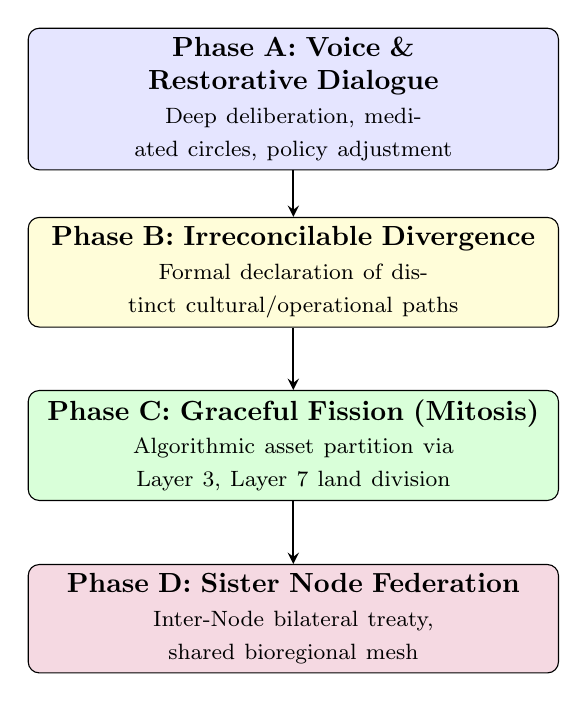
\begin{tikzpicture}[auto, >=stealth]
    \node [rectangle, draw, rounded corners, fill=blue!10, text width=6.5cm, text centered, minimum height=1cm] (voice) at (0, 0) {\textbf{Phase A: Voice \& Restorative Dialogue} \\ \footnotesize Deep deliberation, mediated circles, policy adjustment};
    \node [rectangle, draw, rounded corners, fill=yellow!15, text width=6.5cm, text centered, minimum height=1cm] (divergence) at (0, -2.2) {\textbf{Phase B: Irreconcilable Divergence} \\ \footnotesize Formal declaration of distinct cultural/operational paths};
    \node [rectangle, draw, rounded corners, fill=green!15, text width=6.5cm, text centered, minimum height=1cm] (fission) at (0, -4.4) {\textbf{Phase C: Graceful Fission (Mitosis)} \\ \footnotesize Algorithmic asset partition via Layer 3, Layer 7 land division};
    \node [rectangle, draw, rounded corners, fill=purple!15, text width=6.5cm, text centered, minimum height=1cm] (mesh) at (0, -6.6) {\textbf{Phase D: Sister Node Federation} \\ \footnotesize Inter-Node bilateral treaty, shared bioregional mesh};
    
    \draw [->, thick] (voice) -- (divergence);
    \draw [->, thick] (divergence) -- (fission);
    \draw [->, thick] (fission) -- (mesh);
\end{tikzpicture}
\caption{The lifecycle of graceful node fission (biological mitosis).}
\label{fig:node-fission}
\end{figure}

When a substantial faction within a Node determines that its core cultural, spiritual, or agricultural vision can no longer align with the Genesis Compact, it does not launch an internal coup. It initiates the \textit{Graceful Fission Protocol}:
\begin{enumerate}
    \item \textbf{Notice of Mitosis:} The diverging group files a formal petition in Layer~5, triggering a mandatory three-month reflection and mediation window.
    \item \textbf{Thermodynamic Asset Partitioning:} If reconciliation is not desired, the Layer~3 ledgers and Layer~4 Orchestrators calculate an equitable, mathematically verified partition of pooled capital, movable tools, solar infrastructure, and seed banks, proportionate to historical stewardship contributions and human need.
    \item \textbf{Spawning the Sister Node:} The departing group triggers Vector~3 of the Genesis Protocol (Chapter~9: Direct Layer~6 Mesh Expansion), acquiring adjacent or regional land under a new Community Land Trust to birth an autonomous Sister Node.
    \item \textbf{Bilateral Mesh Treaty:} The parent and sister nodes conclude an inter-node bilateral treaty, maintaining digital mesh interconnection, reciprocal emergency mutual aid, and open visiting rights, transforming an inevitable human conflict into a thriving, polycentric bioregional federation.
\end{enumerate}

\subsection{Neighborhood Assemblies vs. Technocratic Meritocracy}

A critical danger during bringup is the emergence of a technocratic gamer elite. If high-ranking Oasis players behave as self-appointed digital governors, the community will fracture into resentment.

The Sovereign Stack enforces strict anti-technocratic safeguards:
\begin{itemize}
    \item \textbf{The Primacy of the Neighborhood Assembly:} Sovereign political authority is anchored in the in-person, open Neighborhood Assembly \parencite{bookchin1982}. Non-gamers, elders, tenants, and youth possess equal voice and equal voting power with the most seasoned simulation players.
    \item \textbf{Gamers as Servant Facilitators:} Oasis players do not make decisions on behalf of the community. Their role is strictly logistical and consultative: they use their digital twin models to run predictive impact assessments for the assembly (e.g., showing projected thermodynamic trade-offs of different water harvesting layouts or solar arrays). They present options; the assembly decides.
    \item \textbf{Unmediated Spaces:} Under the Protocol of Refusal, the assembly may designate communal halls, dining spaces, gardens, and sacred grounds as permanently unmediated spaces, where all sensors, microphones, cameras, and data collection are strictly banned.
\end{itemize}


\section{From Game to Gateway: The Living Onboarding Pipeline}

In the final phase of collective bring-up, Oasis drops the commercial facade entirely. It ceases to be marketed as a commercial entertainment product and is recognized for what it truly is: the universal Semantic Interface (Layer~6) and educational onboarding gateway of The Collective \parencite{girard2013}.

The simulation remains perpetually active as a living digital twin. Before a physical community undertakes a hazardous real-world project---such as digging a keyline swale across a fragile watershed or rewiring a 480V three-phase solar microgrid---the community tests and rehearses the procedure inside the Oasis engine against simulated storm events and equipment failures. 

For newcomers seeking to transition out of the capitalist rat race, Oasis serves as the welcoming sandbox. Legacy citizens acquire foundational skills, build verified trust with living neighbors, and earn their first Verifiable Credentials in a risk-free digital environment. When they finally walk through the gates of a physical Sovereign Node, they are not strangers or unskilled laborers; they are already sovereign Stewards returning home to a world they have already helped build.
